% !TeX root = ../../tfg.tex
% !TeX encoding = utf8
%
%*******************************************************
% Contenido del artículo 1: Definiciones primeras
%*******************************************************

\section{Definiciones primeras}\label{ch:articulo:sec:defincionesPrimeras}  

Comenzaremos presentando definiciones básicas sobre redes neuronales. 


\begin{definicion}[Función de activación ] \label{def:funcion_activacion_articulo}
    Una función  $\psi: \R \longrightarrow [0,1]$ es una \textbf{ función de activación} si  cumple las siguientes propiedades:
    \begin{enumerate}[label=(\roman*)]
        \item Es no decreciente.
        \item $\lim _{x \rightarrow \infty} \psi(x) = 1
        $.
        \item $\lim _{x \rightarrow -\infty} \psi(x) = 0$.
    \end{enumerate}  
   
    Ejemplos comunes de funciones de activación son

    %%% Nota sobre funciones activación más democráticas que otras
    \marginpar{\textbf{Observación sobre la idoneidad de cada función activación:}
    Se probará la convergencia de las redes neuronales independientemente de la función de activación seleccionada. Cabe entonces la pregunta
    ¿Existen funciones de activación más democráticas que otras?
    }

    % Imágenes de la función indicadora 
    \begin{figure}[h]
        \centering
        \begin{subfigure}[t]{0.47\textwidth}
            \centering
            \includegraphics[width=\textwidth]{
                articulo_rrnn_aproximadores_universales/función_indicadora_l_0.png}
            \caption{Función indicadora $\lambda_0 = 0$}  
            \label{fig:función_indicadora}
        \end{subfigure}
        \hfill
        \begin{subfigure}[t]{0.47\textwidth}  
            \centering 
            \includegraphics[width=\textwidth]{articulo_rrnn_aproximadores_universales/función_umbral_lineal.png
            }
            \caption{Función umbral $w=(2)$, $t=1$}    
            \label{fig:función_umbral_lineal}
        \end{subfigure}
        \begin{subfigure}[t]{0.47\textwidth}   
            \centering 
            \includegraphics[width=\textwidth]{articulo_rrnn_aproximadores_universales/función_rampa.png}
            \caption{Función rampa} 
            \label{fig:funciones_rampa}
        \end{subfigure}
        \hfill
        \begin{subfigure}[t]{0.47\textwidth}   
            \centering 
            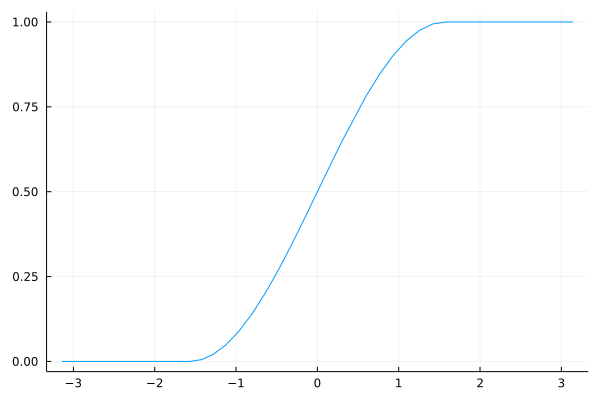
\includegraphics[width=\textwidth]{articulo_rrnn_aproximadores_universales/cosineSquasherSinTitulo.png}
            \caption{\textit{Cosine Squasher}}   
            \label{fig:cosine_squasher}
        \end{subfigure}
        \caption{Ejemplos de funciones de activación} 
        \label{fig:EjemplosFunciónActivación}
    \end{figure}

    \begin{itemize}
        \item \textbf{Funciones umbral} \ref{fig:función_umbral_lineal}:
        Una función umbral, es una función booleana monótona $\psi_w: \{0,1\}^n \longleftarrow \{0,1\},$ 
        donde para $w \in \R^n$, $t \in \R$ fijos se
        satisface que 
        \begin{equation}
            \psi_w(x) = \left\{
                \begin{array}{lcc}
                    1, &   si  & w \cdot x \geq t \\
                    0, &  si & w \cdot x < t\\
                    \end{array}
            \right.
        \end{equation}
        
        \item \textbf{Funciones indicadoras} \ref{fig:función_indicadora}: $\psi(\lambda) = 1_{\{\lambda > \lambda_0\}}$ con $\lambda_0 \in \R$. 
        \item \textbf{Función rampa} \ref{fig:funciones_rampa}: $\psi(\lambda)  = \lambda 1_{\{0 \leq \lambda \leq  1\}} + 1_{\{\lambda > 1\}}.$
    
        \item \textbf{La función \textit{cosine squasher}} de Gallant and White 
        \ref{fig:cosine_squasher} (1988) \cite{Gallant88thereexists}. 
        \begin{equation*}
    \psi(\lambda )= \left(1 + cos\left(\lambda + 3 \frac{\pi}{2} \right) \frac{1}{2}\right) 
     1_{\{\frac{-\pi}{2} \leq \lambda \leq  \frac{\pi}{2}\}}
     +
     1_{\{ \frac{\pi}{2} < \lambda \}}.
    \end{equation*}
    \end{itemize}

   Notemos que así definidas las funciones de activación son medibles, ya que la imagen inversa de un abierto de $[0,1]$ siempre será un conjunto medible de  $\R$  (capítulo 7  página 77 \cite{nla.cat-vn1819421}).
    
    Cabe destacar que la definición tomada es la propuesta en \cite{HORNIK1989359} y que existen
    otras posibles definiciones menos restrictivas con las que también se ha probado la convergencia universal,
    por ejemplo podrían aceptarse funciones de activación no continuas \cite{FUNAHASHI1989183},  
    o como 
    en \cite{DBLP:journals/corr/SonodaM15} con funciones de activación no polinómicas no acotadas. 
    \textcolor{red}{A priori no debería de ser equivalentes entre ellas y será necesario un estudio más 
    profundo para establecer \textit{cuáles son las más democráticas}}
    %TODO añadir sección 

\end{definicion}



Para cualquier natural $r$ mayor que cero  denotaremos por $A^r$ al conjunto de todas 
las \textbf{funciones afines} de $\R^r$ a $\R$. Es decir el conjunto de funciones de la forma 
$A(x) = w \cdot x + b$ donde $x$ y $w$ son vectores de $\R^r$,  $b \in \R$ es un escalar y $\cdot$ representa el producto 
usual de escalares.  
    


En este contexto, $x$ corresponde al vector entrada de la red neuronal, $w$ los pesos de la red
que se multiplicarán con $x$ en la capa intermedia y $b$ el sesgo. 

Nótese que faltaría componer la función afín con una función de activación para obtener lo que hemos definido 
como un perceptrón. 
 % Nota margen sobre que abstrae esta estructura
 \marginpar{\textbf{Idea tras la definición de $\pmc$.}
 Nótese que lo que se ha definido es la clase de las redes 
 neuronales de una capa oculta y salida de una dimensión.
 Donde cada sumatoria representa una neurona en la capa oculta.
 }

\begin{definicion} [Formalización de una red neuronal de una capa oculta y salida real]
    Para cualquier función Borel medible $G$, definida de $\R$ a $\R$ y cualquier natural positivo
    $r \in \N$ se define a la clase de funciones $\pmc$ como 

    \begin{equation}
        \begin{split}
        \pmc = 
        \{ 
            & f: \R ^r \longrightarrow \R / \quad
            f(x)=\sum_{j = 1} ^q (
            \beta_j G(A_{j}(x)), \\
            & x  \in \R ^r, \beta_j \in \R, A_{j}\in A^r,q \in \N
            )
        \}.
        \end{split}
    \end{equation}
\end{definicion}

Con esta misma idea 
se define la siguiente estructura que generaliza a la familia $\pmc.$  
   
   % Idea intuitiva 
   \marginpar{\textbf{Motivación de la definición de $\pmcg$.}
   En un principio será más fácil demostrar que esta clase de funciones es densa en el espacio de funciones continuas.
   De esta manera este conjunto actuará de nexo de unión entre las funciones continuas y las redes neuronales facilitando las demostraciones.
   }
\begin{definicion} [Forma normal generalizada]\label{def:articulo_abstracción_rrnn}
    
    \begin{equation} 
        \begin{split}
        \sum \prod^r(G) = \{ 
        &f: \R^r \longrightarrow \R / \quad
        f(x) = \sum_{j = 1} ^q  \beta_j \prod_{k=1}^{l_j}
        G(A_{jk}(x)), \\
        &x  \in \R^r, \beta_j \in \R, A_{jk}\in A^r; l_j,q \in \N
        )
        \}.
    \end{split}
    \end{equation}  

 
    Notemos que $\pmc$ se recupera en el caso particular en el que $l_j = 1$ para todo $j$.
    Los elementos de $\pmcg$ son combinaciones lineales de productos finitos de neuronas. 

\end{definicion}


\subsection{ Reflexión sobre la relevancia de la función de activación}  

La función de activación $G$ es clave en el proceso de aprendizaje.
Por una parte nótese que como $A^r$ es un espacio afín, lo que se está haciendo es 
aproximar una función medible a partir de combinaciones lineales de \textit{rectas} evaluadas mediante $G$. 
 
\begin{figure}[h!]
    \includegraphics[width=\textwidth]{articulo_rrnn_aproximadores_universales/ejemploAproximaciónCurvasPorRectas.jpeg}
    \caption{Ejemplo de curva aproximada por perceptrones multicapa \cite{alma991008058419704990}.}
    \label{img:def_esenciales_ejemplo_curva_aproximada_percentrón_multicapa}
\end{figure}

Por otra parte, la función de activación acota la imagen de una aplicación afín, esta limitación 
es de total relevancia ya que permite una interpretación previamente convenida. 
Decimos por ende que es la causante del \textit{aprendizaje}.     

Por si el comentario no ha resultado claro procedamos a dar un ejemplo:   
Supongamos que nos hallamos frente a un problema de clasificación de dos clases y que la función de activación
tomada es una función umbral que toma valores cero o uno. Define por tanto esta función una separación de clases. 
De otra manera, de solo existir la función afín sin una transformación de la salida, el codominio serían 
todos los número reales donde a priori no se explicita una asignación de clase.  

Introducimos a continuación la notación de los conjuntos de funciones que seremos capaces de aproximar.  

Denotamos por  $\fC$ al conjunto de funciones continuas con dominio en $\R^r$ y codominio $\R$,
por  $\fM$ al conjunto de todas las funciones Borel medible de $\R^r$ a $\R$. 
y por $B^r$ a la $\sigma$-álgebra de Borel en $\R ^r$. 

En lo que respecta a definiciones anteriores, $\pmc$ y $\pmcg$ pertenecen a 
$\fM$ para cualquier función Borel-medible $G$. Si $G$ es continua entonces 
$\pmc$ y $\pmcg$ pertenecen a $\fC$. Tengamos presente que $\fC$ es un subconjunto
de $\fM$.  

De ahora en adelante nos referiremos a Borel-medible como medible. 
  

\subsection{ Reflexión sobre el tipo de funciones que se pueden aproximar}

La existencia de funciones no medibles manifiesta una limitación
de la formalización actual de las redes neuronales que plantea las siguientes 
preguntas: 
\begin{enumerate}
    \item ¿Supone la existencia de este tipo de funciones una verdadera limitación a nivel práctico?
    \item ¿Se podría construir alguna arquitectura que sí que las aproximara?
\end{enumerate}  

Continuando con el hilo de la segunda cuestión, si se carece de un espacio vectorial, 
de una medida,  ¿Cómo se podría construir una sucesión de funciones que se aproxime?
Quizás habría que buscar características más intrínsecas del problema en cuestión, 
razonamientos topológicos.

\begin{definicion} [Subconjunto denso]
    % Explicación de denso
    \reversemarginpar 
    \marginpar{ \textbf{Idea intuitiva conjunto denso.}
        Si $S$ es denso en $T$, 
        a nivel intuitivo sería decir que los elementos de $S$ son capaces de aproximar cualquier elemento de $T$
        con la precisión que se desee. 
    }
    \normalmarginpar
    Dado un subconjunto $S$ de un espacio métrico $(X, \rho)$, se dice que $S$ es denso por la distancia $\rho$
    en subconjunto $T$ si para todo $\epsilon$ positivo y cualquier $t \in T$ existe un $s \in S$ tal 
    que $\rho(s,t) \leq \epsilon$. 
\end{definicion}

Un ejemplo habitual sería en el espacio métrico $(\R, |\cdot|)$ con $|\cdot|$ el valor absoluto, el subconjunto 
$T = \R$ y $S$ los números irracionales, $S = \R \setminus \Q$. 


\begin{definicion} 
    Un subconjunto $S$ de $\fC$ se dice que es \textbf{uniformemente denso para compactos} en  $\fC$
    si para cada subconjunto compacto $K \subset \R^r$ se tiene que $S_K$ es denso según $\rho_K$ en $\fC$
    donde $\rho_K$ está definida como sigue.
    Para cualquier $f,g \in \fC$ 
    \begin{equation}
        \rho _ K (f,g) = \sup_{x \in K} |f(x) - g(x)|.
    \end{equation}

      % Explicación de uniformemente denso
      
      \marginpar{
          \textbf{Concepto intuitivo  de uniformemente denso para compactos }
          lo que indica es que \textit{controlamos} cuánto de cerca
          están dos funciones sea cual sea cualquier punto del compacto en que evaluemos.
      }
      
\end{definicion}

\begin{definicion}
    Una serie de funciones $\{f_n\}$ \textbf{converge uniformemente a una función $f$ sobre compactos} si para 
    cada  conjunto compacto $K \subset \R^r$  se cumple que
    \begin{equation}
        \rho_k (f_n, f) \longrightarrow 0 \text{ cuando } n \longrightarrow \infty.
    \end{equation} 
\end{definicion}

